
\de{ĐỀ THI GIỮA HỌC KỲ I NĂM HỌC 2022-2023}{THPT Nguyễn Hữu Huân}

\begin{bt}%[Dự án đề kiểm tra GHKI NH22-23- Le Hung Thang]%[0T7B2-1]
	 Cho đồ thị của hàm số bậc hai $f(x)$. Tìm tập nghiệm của bất phương trình tương ứng.
\begin{listEX}[2]
	\item $f(x) \geq 0$\\
	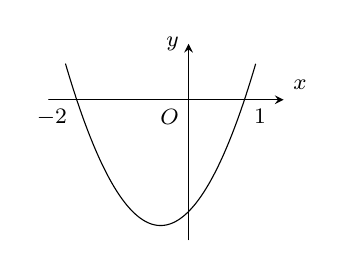
\begin{tikzpicture}[>=stealth,line join=round,line cap=round,font=\footnotesize,scale=0.71]
		\draw[->] (-2.5,0)--(1.7,0)node[above right]{$x$};
		\draw[->] (0,-2.5)--(0,1)node[left]{$y$};
		\fill (0,0)node[below left]{ $O$};
		\draw[black,samples=150,smooth,domain=-2.2:1.2] plot(\x,{(\x)^2+(\x)-2});
		\draw (-2,0)node[below left]{$-2$} (1,0)node[below right]{$1$};
	\end{tikzpicture}
	\item $f(x)<0$\\
	\begin{tikzpicture}[>=stealth,line join=round,line cap=round,font=\footnotesize,scale=0.71]
		\draw[->] (-.5,0)--(4,0)node[above right]{$x$};
		\draw[->] (0,-2.5)--(0,1)node[left]{$y$};
		\fill (0,0)node[below left]{ $O$};
		\draw[black,samples=150,smooth,domain=.45:3.5] plot(\x,{-1*(\x)^2+4*(\x)-4});
		\draw (2,0)node[above]{$2$}	;
	\end{tikzpicture}
\end{listEX}
\loigiai{
	\begin{enumerate}
	\item Dựa vào đồ thị $f(x) \geq 0\Leftrightarrow\hoac{&x\le -2\\&x\ge 1.}$\\
	Vậy tập nghiệm của bất phương trình là $S=(-\infty;-2]\cup[1;+\infty)$.
	\item Dựa vào đồ thị $f(x)<0\Leftrightarrow x\neq 2$.\\
	Vậy tập nghiệm của bất phương trình là $S=\mathbb{R}\setminus\{2\}$.
	\end{enumerate}
}
\end{bt} 

\begin{bt}%[Dự án đề kiểm tra GHKI NH22-23- Le Hung Thang]%[0T7B2-1]
 Định $m$ để bất phương trình $-x^2+2(m+1) x-2 m-2 \leq 0$ có tập nghiệm là $\mathbb{R}$.
\loigiai{
	Ta có 	$\Delta'=(m+1)^2-(-1)(-2m-2)= m^2-1$.\\
	Yêu cầu bài toán thỏa mãn khi
	\allowdisplaybreaks
	$\begin{aligned}[t]
	\Delta'\le 0 \Leftrightarrow &\, m^2-1\le 0\\
	\Leftrightarrow	& \, |m|\le 1\Leftrightarrow -1\le m\le 1.
	\end{aligned}$\\
	Vậy $m\in[-1;1]$ thỏa yêu cầu bài toán.
	}
\end{bt}

%E:\DU AN TEX HOA 2023\6 du an de HK2 Toan 10 HCM\dot7\10_GK2_NGUYENHUUHUAN.tex
\begin{bt}%[Dự án đề kiểm tra GHKI NH22-23- Le Hung Thang]%[0T7K3-2]
Giải phương trình $\sqrt{15-2 x-x^2}-x=-3$.
	\loigiai{
	\allowdisplaybreaks
	\begin{eqnarray*}
	&&\sqrt{15-2 x-x^2}-x=-3\\
	&\Leftrightarrow&\sqrt{15-2 x-x^2}=x-3\\
	&\Leftrightarrow&\heva{&x-3\ge 0\\&15-2x-x^2=(x-3)^2}\\
	&\Leftrightarrow&\heva{&x\ge 3\\&2x^2-4x-6=0}\\
	&\Leftrightarrow&\heva{&x\ge 3\\&\hoac{&x=-1\\&x=3}}\\
	&\Leftrightarrow&x=3.
	\end{eqnarray*}
	Vậy $x=3$ là nghiệm của phương trình.
	}
\end{bt} 

%E:\DU AN TEX HOA 2023\6 du an de HK2 Toan 10 HCM\dot7\10_GK2_NGUYENHUUHUAN.tex
\begin{bt}%[Dự án đề kiểm tra GHKI NH22-23- Le Hung Thang]%[0T8K1-3]
Từ các chữ số $0;\,1;\,2;\,3;\,4;\,5;\,6$ có thể lập được bao nhiêu số tự nhiên lẻ có $3$ chữ số khác nhau đôi một và một trong hai chữ số đầu tiên là số $3$?
	\loigiai{
	Gọi số tự nhiên thỏa đề có dạng $n=\overline{abc}$. Theo yêu cầu bài toán ta có hai trường hợp sau
	\begin{itemize}
	\item Trường hợp $a=3$ hay $n=\overline{3bc}$\\
	 Chọn $c\in\{1,5\}$ có hai cách chọn (vì $n$ là số lẻ).\\
	 Chọn $b\in\{0;1;2;4;5;6\}\setminus\{c\}$ có năm cách chọn.\\
	 Do đó có $2\cdot 5=10$ số thỏa trường hợp này.
	 \item Trường hợp $b=3$ hay $n=\overline{a3c}$\\
	 Chọn $c\in\{1,5\}$ có hai cách chọn (vì $n$ là số lẻ).\\
	 Chọn $a\in\{1;2;4;5;6\}\setminus\{c\}$ có bốn cách chọn.\\
	 Do đó có $2\cdot 4=8$ số thỏa trường hợp này.
	\end{itemize}
	Vậy có $10+8=18$ số thỏa yêu cầu bài toán.
	}
\end{bt}

%E:\DU AN TEX HOA 2023\6 du an de HK2 Toan 10 HCM\dot7\10_GK2_NGUYENHUUHUAN.tex
\begin{bt}%[Dự án đề kiểm tra GHKI NH22-23- Le Hung Thang]%[0T5B4-6]%[0T9B2-2]%[0T9K2-6]%%% Nhờ thầy PB gắn lại giúp ID câu a)
	Trong mặt phẳng $Oxy$, cho tam giác $A B C$ với $A(1;2)$, $B(3;-4)$, $C(0;-1)$.
	\begin{enumerate}
	\item Tìm côsin của góc giữa hai véc-tơ $\vec{A B}, \vec{A C}$.
	\item Viết phương trình tổng quát của đường thẳng $BC$.
	\item Cho đường thẳng $d\colon\heva{&x=-4-2 t\\&y=-3+t}\,\,(t\in \mathbb{R})$. Tìm tọa độ điểm $M$ trên đường thẳng $d$ biết điểm $M$ cách đều $A$ và $B$.
	\end{enumerate}
	\loigiai{
	\begin{enumerate}
	\item Ta có $\vec{AB}=(2;-6)$, $\vec{AC}=(-1;-3)$.\\
	Suy ra $\cos\left(\vec{AB},\vec{AC}\right)=\dfrac{\vec{AB}\cdot\vec{AC}}{\left|\vec{AB}\right|\cdot\left|\vec{AC}\right|}=\dfrac{2\cdot(-1)+(-6)\cdot(-3)}{\sqrt{40}\cdot\sqrt{10}}=\dfrac{16}{20}=\dfrac{4}{5}$.
	\item Ta có $\vec{BC}=(-3;3)$. Suy ra $BC$ có véc-tơ pháp tuyến là $\vec{n}=(1;1)$.\\
	$BC$ có phương trình tổng quát là
	$$1(x-3)+1(y+4)=0 \Leftrightarrow x+y+1=0.$$
	\item Gọi $M(-4-2t;-3+t)\in d$.\\
	Theo đề bài  \vspace*{-0.5 cm}
	\allowdisplaybreaks
	\begin{eqnarray*}
	& &MA=MB\\
	&\Leftrightarrow&(1+4+2t)^2+(2+3-t)^2=(3+4+2t)^2+(-4+3-t)^2\\
	&\Leftrightarrow&4t^2+20t+25+t^2-10t+25=4t^2+28t+49+t^2+2t+1\\
	&\Leftrightarrow&20t=0\\
	&\Leftrightarrow&t=0.
	\end{eqnarray*}
	Vậy $M(-4;-3)$ thỏa mãn yêu cầu bài toán.
	\end{enumerate}

	}
\end{bt} 

%E:\DU AN TEX HOA 2023\6 du an de HK2 Toan 10 HCM\dot7\10_GK2_NGUYENHUUHUAN.tex
\begin{bt}%[Dự án đề kiểm tra GHKI NH22-23- Le Hung Thang]%[0T9B3-2]%[0T9K3-3]
	\begin{enumerate}
	\item Lập phương trình của đường tròn $(C)$ có tâm $I(3;-2)$ và đi qua điểm $M(-1;1)$.
	\item Cho đường tròn $(C_1)\colon(x+2)^2+(y+2)^2=25$. Viết phương trình tiếp tuyến của $(C_1)$ biết tiếp tuyến song song với đường thẳng $d\colon 4x+3y-11=0$.
	\end{enumerate}
	\loigiai{
	\begin{enumerate}
	\item 
	Vì $(C)$ có tâm $I(3;-2)$ và đi qua điểm $M(-1;1)$ nên $(C)$ có bán kính là $R=IM=\sqrt{(-1-3)^2+(1+2)^2}=5$.\\
	Vậy đường tròn $(C)$ có phương trình là
	$$(x-3)^2+(y+2)^2=25.$$
	\item Đường tròn $(C_1)$ có tâm $I_1(-2;-2)$ và bán kính $R_1=5$.\\
	Gọi $d_1$ là tiếp tuyến của $(C_1)$ thỏa đề bài.\\
	Vì $d_1 \parallel d$ nên phương trình của $d_1$ có dạng $ 4x+3y+C=0$, $(C\neq -11)$.\\
	Điều kiện tiếp xúc
	$$\mathrm{d}(I_1,d_1)=R_1\Leftrightarrow\dfrac{|-8-6+C|}{\sqrt{25}}=5\Leftrightarrow\hoac{&C-14=25\\&C-14=-25}\Leftrightarrow\hoac{&C=39 \quad  \text{(nhận)}\\&C=-11\quad \text{(loại)}.}$$
	Vậy tiếp tuyến của $(C_1)$ thỏa đề bài là $d_1\colon 3x+4y+39=0$.
	\end{enumerate}
	}
\end{bt}

%E:\DU AN TEX HOA 2023\6 du an de HK2 Toan 10 HCM\dot7\10_GK2_NGUYENHUUHUAN.tex
\begin{bt}%[Dự án đề kiểm tra GHKI NH22-23- Le Hung Thang]%[0T7K2-1]
	Một đoạn kẽm dài $6$ mét được cắt ra làm hai phần: một phần uốn thành hình vuông có cạnh bằng $x$ mét, phần còn lại uốn thành hình chữ nhật có chiều dài gấp $3$ lần chiều rộng. Tìm điều kiện của $x$ để diện tích hình chữ nhật lớn hơn diện tích hình vuông (kết quả làm tròn đến hàng phần chục).
	\loigiai{
	Đoạn kẽm uốn thành hình vuông có cạnh là $x$ (m) nên chiều dài đoạn kẽm uốn hình vuông là $4x$ (m).\\
	Điều kiện $0<x<\dfrac{3}{2}$.\\
	Diện tích hình vuông là $x^2$.\\
	Khi đó, chiều dài đoạn kẽm uốn thành hình chữ nhật là $6-4x$ (m).\\
	Gọi $y$ (m) là chiều rộng hình chữ nhật, suy ra $2(y+3y)=6-4x$ hay $y=\dfrac{3}{4}-\dfrac{1}{2}x$.\\
	Diện tích hình chữ nhật là $3y\cdot y=3\cdot\left(\dfrac{3}{4}-\dfrac{1}{2}x\right)^2$.\\
	 Theo đề bài, ta có bất phương trình
	 \allowdisplaybreaks
	 \begin{eqnarray*}
	 	&&3\cdot\left(\dfrac{3}{4}-\dfrac{1}{2}x\right)^2>x^2\\
	 	&\Leftrightarrow&\dfrac{27}{16}-\dfrac{9}{4}x+\dfrac{3}{4}x^2>x^2\\
	 	&\Leftrightarrow&4x^2+36x-27<0\\
	 	&\Leftrightarrow&-9{,}696\approx\dfrac{-9-6\sqrt{3}}{2}<x<\dfrac{-9+6\sqrt{3}}{2}\approx 0{,}696.
	 \end{eqnarray*}
	Kết hợp với điều kiện ta có kết quả làm tròn là $0<x<0{,}7$ (đơn vị của $x$ là mét) thỏa yêu cầu bài toán.
	}
\end{bt} 

